\documentclass{beamer}
\usepackage[edges]{forest}
\usepackage{tikz}
\usepackage{media9}
\usetikzlibrary{arrows.meta, positioning}
\usepackage{graphicx}
\usepackage[utf8]{inputenc}
\usepackage[style=authoryear, backend=biber]{biblatex}
\usepackage{listings}
\usepackage{xcolor}
\usepackage{pdfpages}
\addbibresource{main.bib}

\definecolor{mGreen}{rgb}{0,0.6,0}
\definecolor{mGray}{rgb}{0.5,0.5,0.5}
\definecolor{mPurple}{rgb}{0.58,0,0.82}
\definecolor{backgroundColour}{rgb}{0.95,0.95,0.92}

\lstdefinestyle{CStyle}{
    basicstyle=\ttfamily\footnotesize,
    backgroundcolor=\color{backgroundColour},   
    commentstyle=\color{mGreen},
    keywordstyle=\color{magenta},
    numberstyle=\tiny\color{mGray},
    stringstyle=\color{mPurple},
    basicstyle=\footnotesize,
    breakatwhitespace=false,         
    breaklines=true,                 
    captionpos=b,                    
    keepspaces=true,                 
    numbers=left,                    
    numbersep=5pt,                  
    showspaces=false,                
    showstringspaces=false,
    showtabs=false,                  
    tabsize=2,
    language=C
}

\setbeamertemplate{caption}[numbered]
\renewcommand{\figurename}{Figura}

\usetheme{Boadilla}
\usecolortheme{whale}

\title[Progresso do TCC]{Explorando algoritmos de compressão de dados: teoria, implementação e desempenho}
\author[Gustavo Kadooka]{Gustavo Yujii Silva Kadooka}
\institute[UNESP]{Universidade Estadual Paulista - Câmpus Bauru}
\date{2025}
\logo{\includegraphics[scale=0.14]{imagens/unesp.png}}

\begin{document}

\begin{frame}
    \titlepage
\end{frame}

\begin{frame}{Sum\'ario}
    \tableofcontents
\end{frame}

%--------Se\c{c}\~oes--------
\section{Resumo da proposta}
\begin{frame}{Objetivos}
    \begin{block}{Objetivo geral}
        Analisar comparativamente a eficiência dos algoritmos de compressão de dados clássicos (Huffman, LZ77, LZW, GZIP), focando na taxa de compressão e tempo de execução.
    \end{block}
    \begin{block}{Objetivos específicos}
        \begin{itemize}
            \item Descrever os princípios teóricos dos algoritmos selecionados.
            \item Implementar os algoritmos e testar em diferentes tipos de arquivos.
            \item Fornecer recomendações para a escolha do algoritmo mais adequado.
        \end{itemize}
    \end{block}
\end{frame}

\begin{frame}{Cronograma}
    \begin{figure}
        \caption{Cronograma atualizado}
        \centering
        \resizebox{\textwidth}{!}{
            \begin{tabular}{|c|c|c|c|c|c|c|c|}
                \hline
                \textbf{Etapas} & \textbf{ABR} & \textbf{MAIO} & \textbf{JUN} & \textbf{JUL} & \textbf{AGO} & \textbf{SET} & \textbf{OUT} \\
                \hline
                Levantamento bibliográfico & X & X & X & X & X & X & X \\
                \hline
                Desenvolvimento \textit{back-end} & X & X & X & X &   &   &   \\
                \hline
                Desenvolvimento \textit{front-end} &   & X & X & X & X &   &   \\
                \hline
                Testes e análise de desempenho &   &   & X & X & X &   &   \\
                \hline
                Escrita da monografia &   & X & X & X & X & X & X \\
                \hline
            \end{tabular}
        }
        \vspace{0.5em}
        {\footnotesize \textbf{Fonte:} Desenvolvido pelo autor.}
    \end{figure}
\end{frame}

\section{Progresso atual}
\begin{frame}{Atividades Conclu\'idas (abril -- maio)}
    \begin{itemize}
        \item Levantamento bibliogr\'afico conclu\'ido em abril.
        \item In\'icio da implementa\c{c}\~ao do \textit{back-end} (API de manipulação de arquivos WAV e BMP e algoritmos Huffman e LZ77).
        \item In\'icio do front-end com GTK (interface b\'asica).
        \item Escrita parcial da monografia (introdu\c{c}\~ao e fundamenta\c{c}\~ao te\'orica).
    \end{itemize}
\end{frame}

\begin{frame}{Levantamento bibliográfico}
    Algumas das referências bibliográficas utilizadas até o momento são:
    \begin{block}{Artigos Clássicos}
        \textcolor{blue} {
            ~\cite{hartley1928}
            ~\cite{shannon1948}
            ~\cite{huffman1952method}
            ~\cite{ziv1977universal}
            ~\cite{welch1984technique}
        }
    \end{block}
    \begin{block}{Novos algoritmos de compressão}
        \textcolor{blue} {
            ~\cite{alakuijala2016brotli}
            ~\cite{collet2016zstandard}
            ~\cite{wavenet}
        }
    \end{block}
    \begin{block}{Outros}
        \textcolor{blue} {
            ~\cite{salomon2007data}
            ~\cite{deutsch1996gzip}
        }
    \end{block}
\end{frame}

\begin{frame}{Back-End}
\begin{forest}
for tree={
  align=left,
  font=\scriptsize,
  grow'=0,
  draw,
  rounded corners,
  fill=blue!10,
  edge path={
    \noexpand\path [draw, \forestoption{edge}]
    (!u.parent anchor) -- +(2pt,0) |- (.child anchor)\forestoption{edge label};
  },
  parent anchor=east,
  child anchor=west,
  l sep+=1pt,
  s sep=0pt,
  anchor=west,
  calign=first,
  inner sep=0.5pt,
  fit=band,
}
[project
  [build]
  [data
    [input
      [bmp\_example.bmp, fill=red!30]
      [txt\_example.txt, fill=red!30]
      [wav\_example.wav, fill=red!30]
      [\dots, fill=yellow!30]
    ]
    [output
      [huffman0
        [bmp\_example\_huffman0.bmp.GK, fill=green!30]
        [bmp\_example\_huffman0decompressed.bmp, fill=red!30]
        [txt\_example\_huffman0.txt.GK, fill=green!30]
        [txt\_example\_huffman0decompressed.txt, fill=red!30]
        [wav\_example\_huffman0.wav.GK, fill=green!30]
        [wav\_example\_huffman0decompressed.wav.GK, fill=red!30]
        [\dots, fill=yellow!30]
      ]
      [huffman1
        [\dots, fill=yellow!30]
      ]
      [huffman2
        [\dots, fill=yellow!30]
      ]
      [lz77
        [\dots, fill=yellow!30]
      ]
      [lwz 
        [\dots, fill=yellow!30]
      ]
      [gzip
        [\dots, fill=yellow!30]
      ]
    ]
    [\dots, fill=yellow!30]
  ]
]
\end{forest}
\end{frame}

\begin{frame}{Back-End}
\begin{forest}
for tree={
  align=left,
  font=\scriptsize,
  grow'=0,
  draw,
  rounded corners,
  fill=blue!10,
  edge path={
    \noexpand\path [draw, \forestoption{edge}]
    (!u.parent anchor) -- +(2pt,0) |- (.child anchor)\forestoption{edge label};
  },
  parent anchor=east,
  child anchor=west,
  l sep+=1pt,
  s sep=0pt,
  anchor=west,
  calign=first,
  inner sep=0.5pt,
  fit=band,
}
    [project
        [\dots, fill=yellow!30]
        [include
            [formats
                [bmp.hpp, fill=red!30]
                [wav.hpp, fill=red!30]
            ]
        [huffman
          [huffman.hpp, fill=red!30]
          [huffman\_txt.hpp, fill=red!30]
          [huffman\_wav.hpp, fill=red!30]
          [huffman\_bmp.hpp, fill=red!30]
        ]
        [lz77
          [\dots, fill=yellow!30]
        ]
        [GUI.hpp, fill=red!30]
      ]
        [src
            [formats
              [bmp.cpp, fill=red!30]
              [wav.cpp, fill=red!30]
            ]
            [huffman
              [\dots, fill=yellow!30]
            ]
            [lz77
              [\dots, fill=yellow!30]
            ]
            [python\_graphs
              [generate\_bar\_graph.py, fill=red!30]
              [generate\_box\_plot.py, fill=red!30]
              [generate\_csv.py, fill=red!30]
              [generate\_line\_graph.py, fill=red!30]
              [generate\_scatter\_plot.py, fill=red!30]
            ]
            [GUI.cpp, fill=red!30]
            [main.cpp, fill=red!30]
        ]
        [Makefile, fill=blue!40]
    ]
\end{forest}
\end{frame}

\begin{frame}{Fluxo Geral do Projeto}
\centering
\begin{figure}
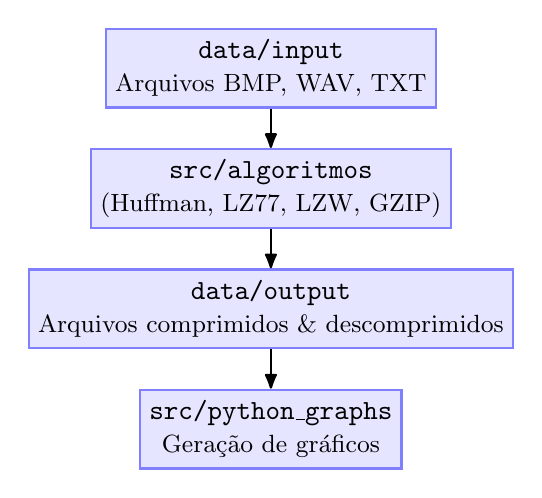
\begin{tikzpicture}[
  node distance=0.5cm and 1cm,
  box/.style={rectangle, draw=blue!50, fill=blue!10, thick, minimum height=1cm, minimum width=1cm, align=center},
  arrow/.style={-{Latex[round]}, thick}
]

\node[box] (input) {\texttt{data/input} \\ \small Arquivos BMP, WAV, TXT};
\node[box, below=of input] (alg) {\texttt{src/algoritmos} \\ \small (Huffman, LZ77, LZW, GZIP)};
\node[box, below=of alg] (output) {\texttt{data/output} \\ \small Arquivos comprimidos \& descomprimidos};
\node[box, below=of output] (graf) {\texttt{src/python\_graphs} \\ \small Geração de gráficos};

\draw[arrow] (input) -- (alg);
\draw[arrow] (alg) -- (output);
\draw[arrow] (output) -- (graf);

\end{tikzpicture}
\vspace{0.5em}

{\small \textbf{Fonte:} Diagrama elaborado pelo autor com base na estrutura de diretórios do projeto.}
\end{figure}
\end{frame}

\begin{frame}[fragile]{Back-End -- API wav.h}
    \begin{lstlisting}[style=CStyle]
class wav {
public:
    struct RIFF_chunk_descriptor {
        char ID[4];
        uint32_t size;
        char format[4];
    } riff_chunk_descriptor;
    struct FMT_subchunk {
        char ID[4];
        ...
    } fmt_subchunk;
    struct DATA_subchunk {
        ...
    } data_subchunk;
    uint8_t* data; 

    int read(std::string filename);
    void print();
};
    \end{lstlisting}
\end{frame}

\begin{frame}[fragile]{Back-End -- API wav.c}
    \begin{lstlisting}[style=CStyle]
int wav::read(std::string filename) {
    FILE *file = fopen(filename.c_str(), "rb");
    if(!file) {
        return -1;
    }
    if(fread(&riff_chunk_descriptor, sizeof(riff_chunk_descriptor), 1, file) != 1) {
        fclose(file);
        return -1;
    }
    if(fread(&fmt_subchunk, sizeof(fmt_subchunk), 1, file) != 1) { ... }
    if(fread(&data_subchunk, sizeof(data_subchunk), 1, file) != 1) { ... }
    data = new uint8_t[data_subchunk.size];
    if(!data) { ... }
    if(fread(data, data_subchunk.size, 1, file) != 1) { ... }
    fclose(file);
    return 0;
}
    \end{lstlisting}
\end{frame}

\begin{frame}{Back-End}
    \begin{center}
        \href{{https://github.com/guhkadoo/unesp/tree/main/Projeto\%20e\%20Implementa\%C3\%A7\%C3\%A3o\%20de\%20Sistemas/GKompress}}{
            \includegraphics[width=0.5\linewidth]{imagens/github}
        }
    \end{center}
\end{frame}

\begin{frame}{Front-End}
    \begin{center}
        \href{https://youtu.be/l5vd6v1kVy0}{
            \includegraphics[width=0.7\linewidth]{imagens/imagem1}
        }
    \end{center}
\end{frame}

\begin{frame}{Front-End}
    \begin{center}
        \href{https://youtu.be/u9ARyP\_xsv8}{
            \includegraphics[width=0.7\linewidth]{imagens/imagem2}
        }
    \end{center}
\end{frame}

\begin{frame}{Testes e análise de desempenho}
\begin{table}[h]
\centering
\begin{tabular}{|l|r|r|r|}
\hline
\textbf{Arquivo} & \textbf{Original (B)} & \textbf{Comprimido (B)} & \textbf{Compressão (\%)} \\
\hline
\texttt{txt\_example5} & 457730 & 269554 & 41,12\% \\
\texttt{txt\_example19} & 88005 & 49819 & 43,40\% \\
\texttt{wav\_example4} & 10543996 & 9748029 & 7,56\% \\
\texttt{bmp\_example2} & 53747850 & 53045595 & 1,31\% \\
\texttt{txt\_example9} & 1503949 & 864639 & 42,50\% \\
\texttt{txt\_example92} & 37189 & 21018 & 43,48\% \\
\texttt{txt\_example2} & 6311 & 3610 & 42,80\% \\
\texttt{txt\_example45} & 80413 & 46081 & 42,69\% \\
\texttt{txt\_example33} & 68654 & 39212 & 42,90\% \\
\texttt{txt\_example70} & 49444 & 28055 & 43,26\% \\
\hline
\end{tabular}
\caption{Exemplo de .csv usando o algoritmo de Huffman com árvore na memória}
\end{table}
\end{frame}

\begin{frame}{Testes e análise de desempenho}
    \begin{center}
        \includegraphics[width=0.8\linewidth]{imagens/file_sizes_huffman0_txt_scatter_plot}
    \end{center}
\end{frame}

\begin{frame}{Testes e análise de desempenho}
    \begin{center}
        \includegraphics[width=0.8\linewidth]{imagens/file_sizes_huffman0_bmp_scatter_plot}
    \end{center}
\end{frame}

\begin{frame}{Testes e análise de desempenho}
    \begin{center}
        \includegraphics[width=0.8\linewidth]{imagens/file_sizes_huffman0_wav_scatter_plot}
    \end{center}
\end{frame}

\begin{frame}{Testes e análise de desempenho}
    \begin{center}
        \includegraphics[width=0.8\linewidth]{imagens/file_sizes_huffman1_txt_scatter_plot}
    \end{center}
\end{frame}

\begin{frame}{Testes e análise de desempenho}
    \begin{center}
        \includegraphics[width=0.8\linewidth]{imagens/file_sizes_huffman2_txt_scatter_plot}
    \end{center}
\end{frame}

\begin{frame}{Testes e análise de desempenho}
    \begin{center}
        \includegraphics[width=0.8\linewidth]{imagens/file_sizes_lz77_txt_scatter_plot}
    \end{center}
\end{frame}


\begin{frame}{Testes e análise de desempenho}
    \begin{center}
        \includegraphics[width=0.8\linewidth]{imagens/file_sizes_huffman0_compression}
    \end{center}
\end{frame}

\begin{frame}{Testes e análise de desempenho}
    \begin{center}
        \includegraphics[width=0.8\linewidth]{imagens/file_sizes_huffman1_compression}
    \end{center}
\end{frame}

\begin{frame}{Testes e análise de desempenho}
    \begin{center}
        \includegraphics[width=0.8\linewidth]{imagens/file_sizes_huffman2_compression}
    \end{center}
\end{frame}

\begin{frame}{Testes e análise de desempenho}
    \begin{center}
        \includegraphics[width=0.8\linewidth]{imagens/file_sizes_lz77_compression}
    \end{center}
\end{frame}

\appendix
\includepdf[pages=-, fitpaper=true, pagecommand={\thispagestyle{empty}}]{monografia.pdf}

\begin{frame}{Progresso de Junho (em andamento)}
    \begin{itemize}
        \item Continuidade do desenvolvimento dos algoritmos (LZW e GZIP).
        \item Testes de compress\~ao com arquivos \texttt{.txt}, \texttt{.bmp} e \texttt{.wav}.
        \item Geração de gráficos com Python.
        \item Consolida\c{c}\~ao de resultados parciais para an\'alise.
    \end{itemize}
\end{frame}

\section{Pr\'oximos Passos}
\begin{frame}{O que vem a seguir (julho em diante)}
    \begin{itemize}
        \item Finalizar implementa\c{c}\~ao do back-end e front-end.
        \item An\'alise estat\'istica dos dados com Python.
        \item Escrita dos resultados e conclus\~ao da monografia.
    \end{itemize}
\end{frame}

\begin{frame}[allowframebreaks, noframenumbering]
    \frametitle{Refer\^encias}
    \printbibliography
\end{frame}

\end{document}
